
\chapter{Ειδικές περιπτώσεις} % Main chapter title

\label{Chapter3} % Change X to a consecutive number; for referencing this chapter elsewhere, use \ref{ChapterX}
Το πρόβλημα vertex cover παρόλο που είναι NP-πλήρης στη γενική περίπτωση σε κάποιες ειδικές περιπτώσεις γράφων είναι δυνατό να λυθεί σε πολυωνυμικό χρόνο. Παρακάτω παραθέτονται κάποιες από αυτές τις ειδικές περιπτώσεις και ορισμένες λύσεις και πορίσματα.
%----------------------------------------------------------------------------------------
%	SECTION 1
%----------------------------------------------------------------------------------------

\section{Bigraphs}

\subsection{Εισαγωγικές έννοιες}

\begin{enumerate}
\item
Διμερής γράφοι:\\
Οι διμερής γράφοι είναι ειδικές περιπτώσεις γράφων όπου οι κόμβοι τους μπορούν να χωριστούν σε δύο ανεξάρτητα σύνολα $\mathcal{U}$ και $\mathcal{V}$ ετσί ώστε κάθε ακμή να ενώνει ένα κόμβο του $\mathcal{U}$ με έναν κόμβο του $\mathcal{V}$. 
\item
Matching:\\
Δεδομένου ενός γράφου $G=(V,E)$ ονομάζουμε matching $Μ$ στον $G$ ένα σύνολο μη γειτονικών ακμών, δηλάδη ακμές που δεν είναι προσκήμενες στον ίδιο κόμβο. Μέγιστο matching ονομάζουμε το σύνολο με τον μέγιστο αριθμό ακμών.
\end{enumerate}
\begin{figure}[H]
\caption{Matching example}
\centering
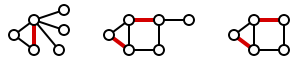
\includegraphics{Figures/match.png}\centering
\end{figure}

\begin{figure}[H]
\caption{Maximum matching example}
\centering
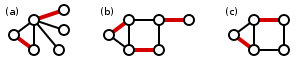
\includegraphics{Figures/max_match.png}\centering
\end{figure}

\subsection{Θεώρημα Konig}

Σε αυτό το είδος γράφων βρίσει εφαρμογή το θεώρημα του Konig το οποίο αναφέρει πως για κάθε διμερή γράφο $G=(V,E)$ ισχύει $\nu(G) = \tau(G)$ όπου\\
$\nu(G) := $ maximum size of a matching in G,\\
$\tau(G) := $ minimum size of a vertex cover in G.

\subsection{Απόδειξη}
\justify
Έστω ένας διμερής γράφος $G = (L, R, E)$ και ένα μέγιστο ταίριασμα $M$. Τότε επειδή κανένας κόμβος ενός vertex cover δεν μπορεί να καλύπτει περισσότερες από δύο ακμές του συνόλου $M$ (διαφορετικά δεν θα ήταν ταίριασμα), ένα vertex cover μεγέθους $|M|$ θα είναι το ελάχιστο vertex cover.\\
Για να δημιουργήσουμε ένα τέτοιο vertex cover, έστω $U$ το σύνολο των μη ταιριασμένων κόμβων του $L$, και $Z$ το σύνολο των ακμών που είτε είναι στο $U$ είτε συνδέονται με αυτό μέσω εναλακτικών μονοπατιών (alternating paths). Τότε το σύνολο $V' = (L \setminus Z) \cup (R \cap Z)$ είναι ένα vertex cover. 

\subsection{Συμπεράσματα}

Οπότε χρησιμοποιόντας τον αλγόριθμο Hopcroft-Karp, ο οποίος βρίσκει ένα μέγιστο ταίριασμα σε ένα διμερή γράφο σε χρόνο $O(|E| \sqrt{|V|})$, μπορούμε έπειτα να υπολογίσουμε το σύνολο $V'$ αποδοτικά.

\begin{figure}[H]
\caption{Maximum matching - minimum vertex cover example}
\centering
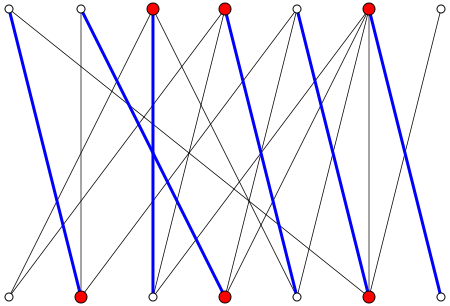
\includegraphics[width=0.4\textwidth]{Figures/KonigTheo.png}\centering
\end{figure}
%----------------------------------------------------------------------------------------
%	SECTION 2
%----------------------------------------------------------------------------------------

\section{Tree graphs}
Για δένδρα υπάρχει ένας άπληστος αλγόριθμος που βρίσκει το ελάχιστο vertex cover σε πολυωνυμικό χρόνο.

\subsection{Εισαγωγικές έννοιες}
Ένα δένδρο είναι ένας μη κατευθυντικός γράφος $G=(V,E)$ που είναι συνεκτικός και δεν έχει κύκλους.

\subsection{Αλγόριθμος}
Η βασική ιδέα του αλγορίθμου είναι η εξής: χρησιμοποιόντας την αναζήτηση πρώτα σε βάθος βρίσκουμε όλα τα φύλλα του δένδρου και έπειτα για κάθε φύλλο επιλέγουμε τον πατέρα του και για κάθε επιλέγουμε κάθε εσωτερικό κόμβο που τα παιδιά του δεν έχουν επιλεχθεί μέχρι να μην υπάρχουν άλλοι κόμβοι να επιλεχθούν.
%----------------------------------------------------------------------------------------
%	SECTION 3
%----------------------------------------------------------------------------------------

\section{Hypergraphs}
\subsection{Εισαγωγικές έννοιες}
Υπεργράφος είναι μια γενίκευση του γράφου όπου μια ακμή μπορεί να συνδέσει περισσότερους από έναν κόμβους. Πιο αυστηρά ένας υπεργράφος $H$ είναι ένα ζευγάρι $H=(X,E)$ όπου $X$ είναι ένα σύνολο του οποίου τα στοιχεία είναι οι κόμβοι και $E$ είναι ένα σύνολο αποτελούμενο από μη κενά υποσύνολα του $X$ και ονομάζονται υπερακμές. 

%----------------------------------------------------------------------------------------
%	SECTION 4
%----------------------------------------------------------------------------------------

\section{Δυικά προβλήματα}

\subsection{Clique}
Ένα clique ενός μη κατευθυντικού γράφου $G=(V,E)$ είναι ένα υποσύνολο των ακμών $C \subseteq V$ τέτοιο ώστε όλοι οι κόμβοι του να είναι γειτονικοί ανά δύο.\\
\\

Δεδομένου ενός μη κατευθυντικού γράφου $G=(V,E)$ ορίζουμε το συμπλήρωμα του ως $\overline{G} = (V, \overline{E})$ όπου $\overline{E} = \{(u,v):u,v \in{V}, u \neq v, (u,v) \notin{E}\}$, τότε αν υπάρχει ένα clique $C$ στον $\overline{G}$ το $V \setminus C$ είναι ένα vertex cover του $G$.

\subsection{Independent set}
